\chapter{陆地生态系统碳循环模型开放式对比框架}
% MDL 模型描述语言
% UDX 统一数据交换表达模型
% UDX JSON Schema
% 基于Web Service的开放式模型对比框架和传统模型对比框架最大的区别就是,前者通过Web Service提供开放式的可共享与重用的模型服务资源和数据服务资源,因此模型和数据资源的开放式接入方法是在网络空间下开展地理模型对比的前提。本章首先分析了地理模型资源的运行特征和描述方法,并在此基础上阐述了模型资源的开放式接入方法;其次讨论了模型所依赖的数据资源的特征及元数据描述方法,并在其上构建了数据资源的开放式接入方法;最后探讨了如何对异构的地理模型资源和数据资源进行数据适配和耦合。

根据第\ref{chap:model}章的分析,陆地生态系统碳循环模型的模拟具有多要素(如GPP、NPP、NEP、Biomass、LAI等)、多站点、数据量大的特点,因此,采用传统的对比方法需要在不同的站点和模拟要素上重复多次对比,对比过程繁琐重复。本章首先设计了一套开放式的、可重用的对比框架,分析了陆地生态系统碳循环模型的对比业务情景,并从中归纳总结出“对比话题——对比方案——对比任务”的三部流程;其次详细探讨了对比过程中的各种可扩展的地理资源组件库,包括有模型服务资源库、数据服务资源库、标准度量资源库、数据重构服务资源库、可视化服务资源库、对比服务资源库,各个资源组件以统一的服务接口暴露出去,实现了对比内容的标准一致性和可扩展性;然后针对陆地生态系统碳循环模型的多样性,设计了分布式的网络系统架构,以支撑异构的碳循环模型的复杂运行环境需求和数据请求与交互需求;最后针对现有的服务化的资源组件,在分布式网络环境下,以科学工作流的方式自动化地调度对比流程。本文所设计的陆地生态系统碳循环模型开放式对比框架如图\ref{fig:CMIP-architecture}所示,以下将分别从对比业务流程分析、开放式地理资源组件库、分布式网络系统架构和开放式对比科学工作流引擎四部分详细阐述。

\begin{figure}
    \centering
    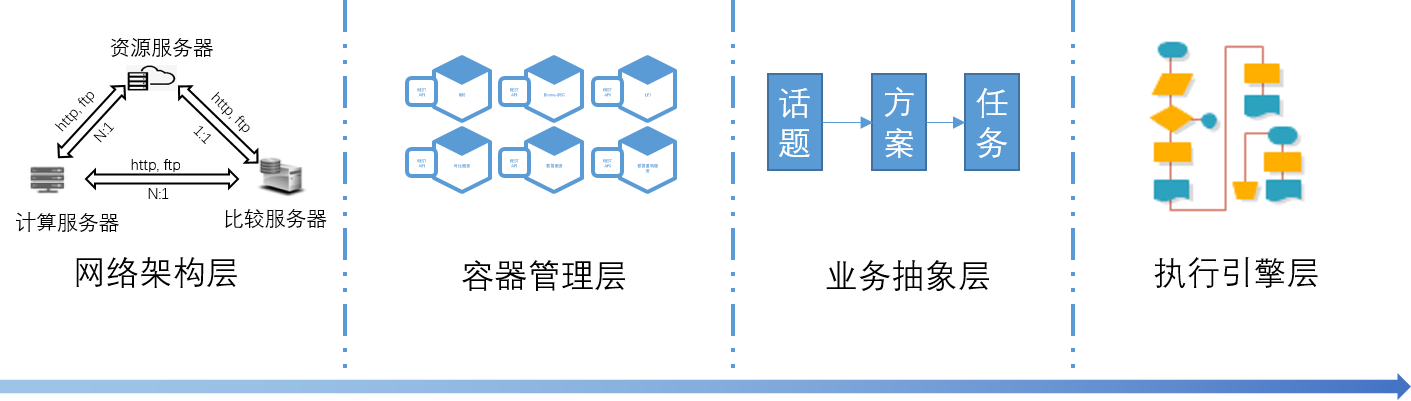
\includegraphics[width=1\textwidth]{CMIP-architecture}
    \caption{陆地生态系统碳循环模型开放式对比框架}
    \label{fig:CMIP-architecture}
\end{figure}

\section{陆地生态系统碳循环模型对比业务流程分析}
\subsection{对比情景分析和总结}
% 对比情景总结 参考CMIP5/CMIP6
% 碳循环模型研究的几个关键问题
在第\ref{sec:model}节中分析过,陆地生态系统碳循环模型的应用广泛,未来的发展方向也主要停留在以下几个关键问题上:
\begin{enumerate}[(1)]
\item \textbf{陆地生态系统碳循环模型对历史植被生长的模拟}
使用历史气象观测资料、CO2浓度数据等分析GPP、NPP、NEP、Biomass等生理生态要素。

\item \textbf{陆地生态系统碳循环模型的未来情景预测}
使用气候模式预测的未来气象资料和CO2浓度分析未来情景中的植被生产力。

\item \textbf{陆地生态系统碳循环模型对气候变化(如温度、降水等)的响应}
分析温度、降水发生变化时,植被生产力对应的变化。

\item \textbf{陆地生态系统碳循环模型的敏感性分析}
分析陆地生态系统碳循环模型中关键参数对模拟结果的决定性影响,分为总体敏感性分析和局部敏感性分析。

\end{enumerate}

而这些模拟情景中,对于实验结果都需要进行对比验证。

\subsection{对比业务抽象和归纳}
% topic solution task
% 可共享 可重用


\section{开放式地理资源组件库}
\subsection{模型服务资源库}
\subsection{数据服务资源库}
\subsection{标准度量资源库}
\subsection{数据重构服务资源库}
\subsection{可视化服务资源库}
\subsection{对比服务资源库}

\section{分布式网络架构设计}
\begin{figure}
    \centering
    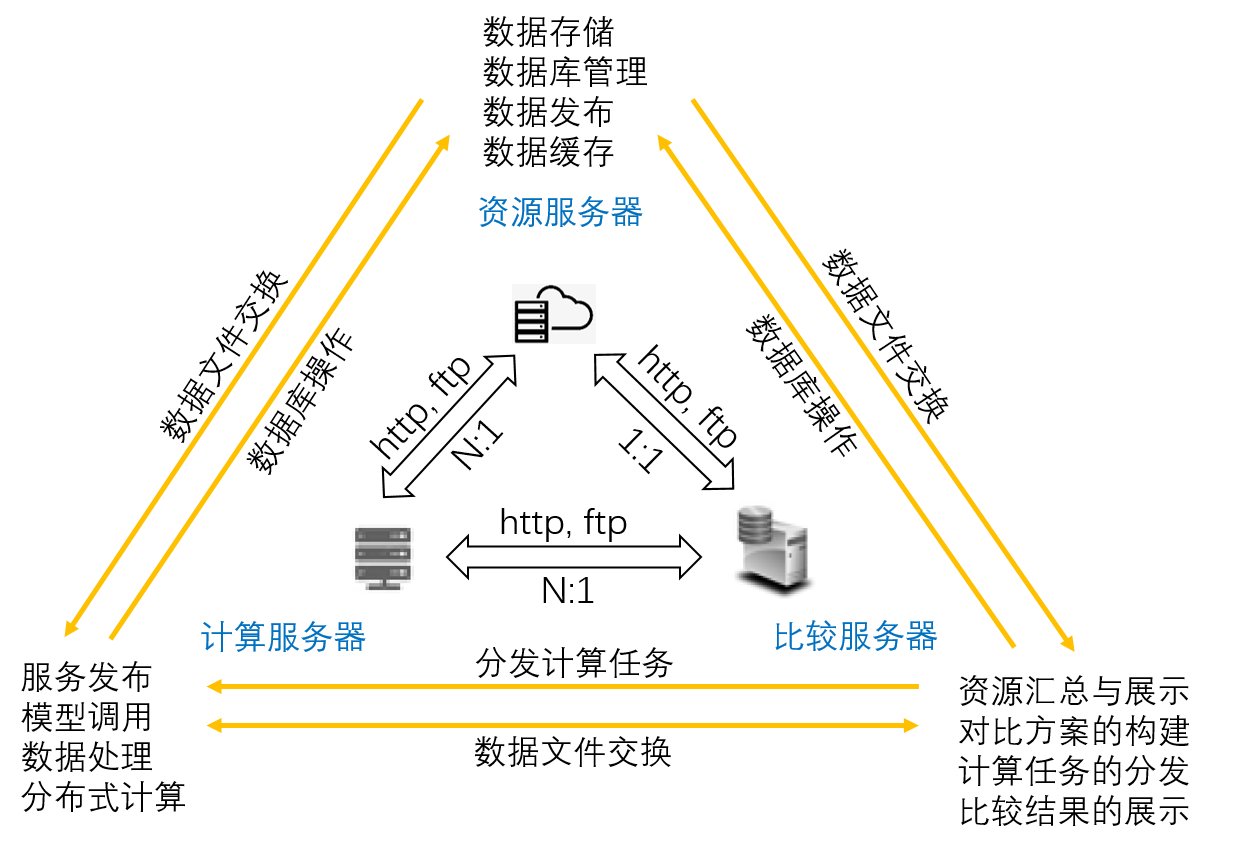
\includegraphics[width=1\textwidth]{network-archecture}
    \caption{分布式网络架构}
    \label{fig:network-archecture}
\end{figure}

\section{开放式对比科学工作流引擎}
\begin{figure}
    \centering
    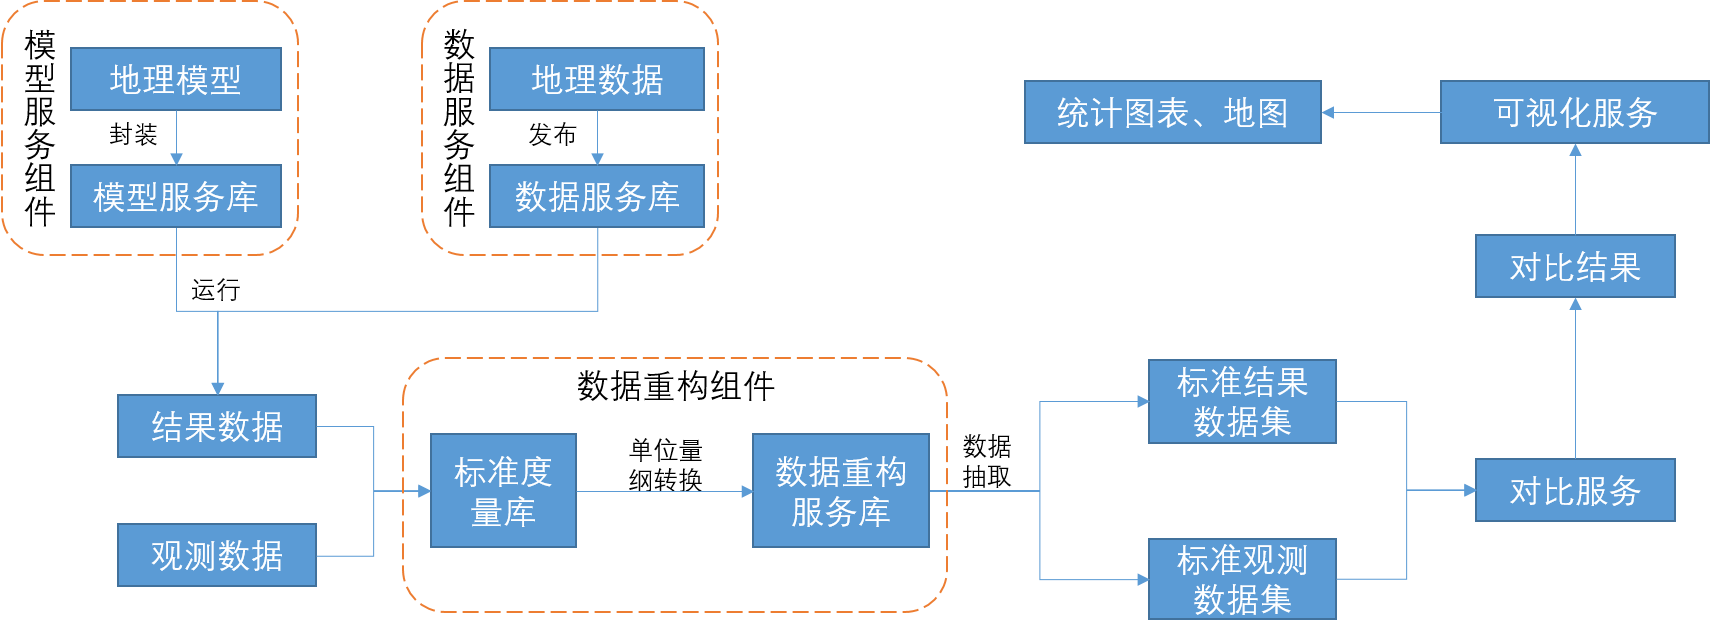
\includegraphics[width=1\textwidth]{workflow}
    \caption{开放式对比科学工作流流程图}
    \label{fig:workflow}
\end{figure}

\begin{figure}
    \centering
    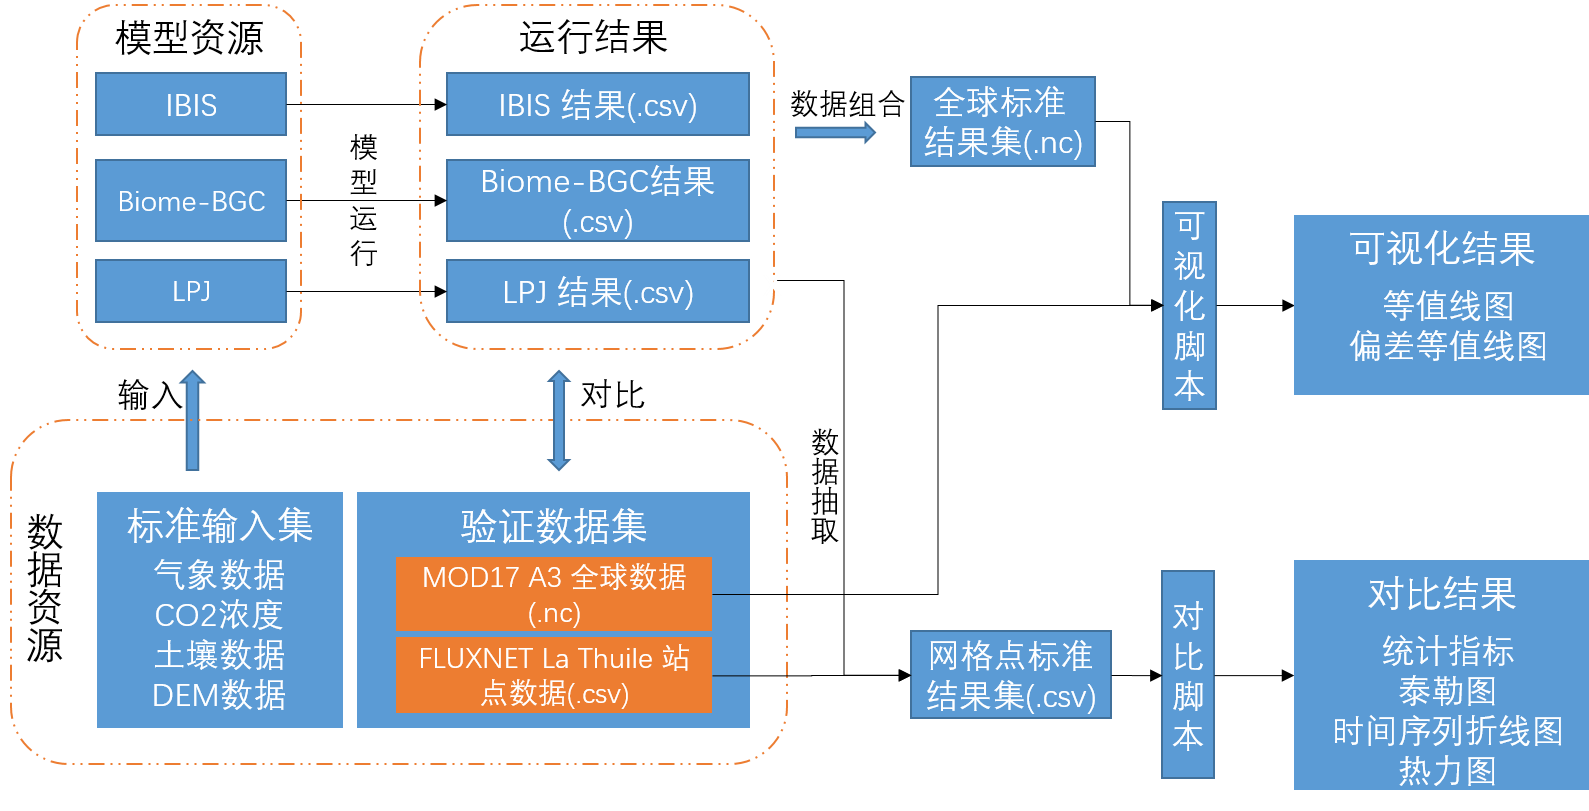
\includegraphics[width=1\textwidth]{workflow-example}
    \caption{以IBIS、Biome-BGC、LPJ三个模型为例的对比科学工作流流程图}
    \label{fig:workflow-example}
\end{figure}

% \section{面向对比的标准度量研究}
% \subsection{面向对比的标准度量及其描述方法}
% \subsection{面向标准度量的数据适配方法}

% \section{模型对比科学工作流引擎}
% % 模型调用-数据缓存-数据重构-数据对比
% \subsection{对比流程分析和归纳}
% \subsection{对比自动化执行引擎}

% \subsection{面向对比的开放式地理资源库}
% \subsubsection{模型资源库}
% % 介绍模型
% \begin{enumerate}[(1)]
% \item \textbf{IBIS}

% \item \textbf{Biome-BGC}

% \item \textbf{LPJ}

% \end{enumerate}


% \subsubsection{数据资源库}
% % 介绍数据
% \begin{enumerate}[(1)]
% \item \textbf{气象数据集}

% \item \textbf{土壤数据集}

% \item \textbf{Fluxdata观测数据集}

% \item \textbf{MODIS GPP产品数据集}

% \item \textbf{模型输出数据集}

% \end{enumerate}
% \subsubsection{标准度量库}
% \subsubsection{数据重构方法库}
% \subsubsection{可视化方法库}
% \subsubsection{对比方法库}
% 介绍对比方法
\begin{enumerate}[(1)]
\item \textbf{泰勒图}

\item \textbf{时间序列折线图}

\item \textbf{箱图}

\item \textbf{热力图}

\item \textbf{偏差等值线图}

\item \textbf{加权超级集合}

\end{enumerate}

\section{本章小结}


